\section{Reti di calcolatori e Internet}

\subsection{Cos'è internet?}
\textbf{Internet} è una rete globale di calcolatori interconnessi, spesso descritta come una 'rete di reti', che comunica utilizzando un insieme comune di protocolli, principalmente la suite TCP/IP.
\subsubsection{Definizioni varie}
\begin{description}[font=\sffamily\bfseries, leftmargin=1cm, style=nextline]
  \item[host] 
    o \textit{sistemi periferici} sistema terminale della rete dove risiedono e vengono eseguite le applicazioni.
  \item[rete di collegamenti]
    o \textit{communication link} il mezzo fisico (es. cavo coassiale, fibra ottica, onde radio) attraverso cui i dati vengono trasmessi tra i nodi della rete.
  \item[commutatori di pacchetti]
    o \textit{packet switch} dispositivi di rete che inoltrano i pacchetti di dati da un collegamento in ingresso a un collegamento in uscita.
  \item[velocità di trasmissione]
    o \textit{transimission rate} velocità con cui i vari tipi di collegamenti si scambiano dati, misurata in \textbf{bit/secondo (bps)} e che rappresenta la capacità del collegamento..
  \item[pacchetto]
    o \textit{packet} unità di dati formata a livello di rete (livello IP), contenente una porzione di dati (che a livello di trasporto, con TCP, è chiamata \textbf{segmento}) e un'intestazione con informazioni di controllo. 
  \item[commutatore di pacchetto]
    dispositivo che riceve un \textbf{pacchetto} su un collegamento in ingresso, lo memorizza temporaneamente e poi lo ritrasmette su un collegamento in uscita. I due tipi principali sono i \textbf{router}, usati nel nucleo della rete per l'instradamento tra reti diverse, e i \textbf{commutatori a livello di collegamento \textit{(link-layer switch)}}, usati nelle reti locali per la commutazione all'interno della stessa rete. 
  \item[percorso]
    o \textit{route} o \textit{path}, sequenza di collegamenti e di commutatori di pacchetto attraversata dal singolo pacchetto. 
  \item[Internet ServiceProvider (ISP)]
    un'organizzazione che possiede e gestisce un insieme di commutatori di pacchetto e di collegamenti, fornendo ai sistemi periferici e ad altre reti l'accesso a Internet.
  \item[applicazioni distribuite]
    o \textit{distributed applications}, più sistemi periferici che si scambiano reciprocamente dati. Vengono eseguite sui sistemi periferici (\textit{host}).
  \item[interfaccia socket]
    o \textit{socket interface} un'interfaccia di programmazione (API) che specifica come un programma eseguito su un sistema periferico può richiedere ai servizi di rete di Internet di recapitare dati a un programma eseguito su un altro sistema periferico.
  \item[protocollo]
    è un insieme di regole rigido, definisce il formato, l’ordine dei messaggi scambiati tra due o più entità in comunicazione, così come le azioni intraprese in fase di trasmissione e/o di ricezione di un messaggio o di un altro evento.
  \item[client e server]
    \textit{host} che richiedono dei servizi (client) e \textit{host} che si occupano di erogare dei servizi (server). Questi ultimi sono spesso collocati in potenti \textbf{data center} per garantire alta disponibilità e prestazioni. 
  \item[reti di accesso]
    o \textit{access network} la rete che connette fisicamente i sistemi periferici al primo \textbf{router} (chiamato \textbf{router di bordo}, o \textit{edge router}) sul percorso verso la rete Internet del provider. 
\end{description}

\subsection{Il nucleo della rete}
Il nucleo della rete è una maglia complessa di commutatori di pacchetti e collegamenti ad alta velocità che interconnettono i sistemi periferici di Internet. La funzione principale del nucleo della rete è quella di instradare i dati tra i sistemi periferici.

\subsubsection{Commutazione di pacchetto}
Le \textit{applicazioni distribuite} scambiano \textbf{messaggi}. Per facilitare la trasmissione e la gestione della rete, la sorgente divide i messaggi più lunghi in unità più piccole chiamate \textit{pacchetti}, che viaggiano attraverso i \textit{commutatori di pacchetto} per raggiungere la destinazione. Ogni pacchetto viene trasmesso sul collegamento fisico alla velocità di trasmissione $R$ (misurata in bit al secondo, bps). Un pacchetto di $L$ bit impiegherà quindi $L/R$ secondi per essere trasmesso completamente sul collegamento.

Una delle tecnologie fondamentali utilizzate dai \textit{commutatori di pacchetto} è la \textbf{trasmissione store and forward}. Secondo questo principio, il commutatore deve ricevere \textbf{completamente} l'intero \textit{pacchetto} prima di iniziare a trasmettere il primo bit verso il collegamento di uscita.

Consideriamo un pacchetto di $L$ bit che viene trasmesso dall'\textit{host} sorgente al primo \textit{router} sul percorso. Se la velocità di trasmissione del collegamento è $R$, il tempo necessario per trasmettere il pacchetto è $L/R$ secondi. Utilizzando la trasmissione store and forward, il router riceverà l'intero pacchetto all'istante $L/R$. Supponendo che anche il collegamento tra il router e l'\textit{host} di destinazione abbia una velocità di trasmissione $R$, il router inizierà a trasmettere il pacchetto verso la destinazione. L'\textit{host} di destinazione riceverà l'intero pacchetto all'istante $L/R$ (trasmissione host-router) + $L/R$ (trasmissione router-host) = $2L/R$.

Generalizzando, considerando un percorso con $N$ collegamenti, ognuno con una velocità di trasmissione $R$, e quindi $N-1$ router intermedi che utilizzano la trasmissione store and forward, il ritardo totale di trasmissione attraverso il percorso (trascurando altri tipi di ritardi come la propagazione) sarà:
\[
  delay = N \frac{L}{R}
\]

Se la sorgente deve inviare $P$ pacchetti in sequenza sullo stesso percorso, il tempo necessario affinché l'ultimo pacchetto raggiunga la destinazione sarà approssimativamente $P \cdot N \frac{L}{R}$, assumendo che ogni pacchetto venga trasmesso solo dopo che il precedente è stato completamente trasmesso.

\textit{Nota:} Se i pacchetti vengono inviati in modo continuo (\textit{pipelining}), l'analisi del ritardo diventa più complessa. Il ritardo per il primo pacchetto rimane $N \frac{L}{R}$, ma i pacchetti successivi arriveranno a intervalli di $\frac{L}{R}$.

Trascurando però i ritardi di propagazione, che rappresentano il tempo impiegato dal segnale per viaggiare attraverso il mezzo fisico.

I commutatori di pacchetto hanno più collegamenti, e per ogni collegamento di output è presente un \textbf{buffer di output} o \textbf{coda di output} per organizzare i pacchetti da inviare su quel collegamento. Questo comporta che i pacchetti subiscono un \textbf{ritardo di accodamento}, il pacchetto deve aspettare che si "liberi il passaggio" per essere trasmesso. Questo ritardo è variabile e dipende dal traffico della rete in un dato momento. Nel caso in cui il buffer sia pieno, avendo una dimensione prestabilita, il pacchetto verrà perso (\textit{packet loss}), verrà eliminato o il pacchetto in arrivo o uno di quelli in coda, dipende dal progettista di rete.

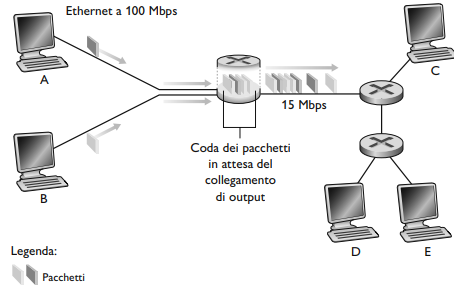
\includegraphics[width=\textwidth, height=6cm, keepaspectratio]{img/commutazione_di_pacchetto.png}

\subsubsection{Commutazione di circuito}
Esiste un altro metodo per scambiare messaggi, ossia la \textbf{commutazione di circuito}. Questo garantisce che le risorse per consentire lo scambio di dati sono \textbf{dedicate} (o \textbf{riservate}), sono quindi esclusivamente allocate per la \textbf{comunicazione}.

Bisogna stabilire un collegamento tra mittente e destinatario, lo chiameremo \textbf{circuito}, attraverso una fase di segnalazione tra i commutatori. A questo circuito verrà riservata una \textbf{velocità di trasmissione costante} (pari a una frazione della capacità del canale).

Ogni \textit{host} della rete è connesso a un commutatore che a sua volta è connesso con gli altri \textit{host} nella rete. Quando un host dovrà comunicare con un altro host, verrà instaurata una \textbf{connessione punto a punto} (\textit{connessione end to end}) \textbf{logica} a loro dedicata.

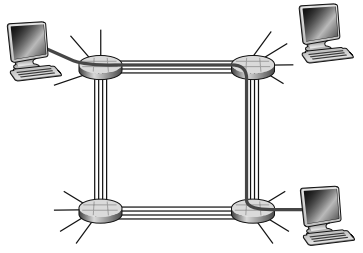
\includegraphics[width=\textwidth, height=6cm, keepaspectratio]{img/commutazione_di_circuito.png}

Un circuito viene implementato tramite \textbf{multiplexing a divisione di frequenza} (\textit{frequency-division multiplexing}) o \textbf{multiplexing a divisione di tempo} (\textit{time-division multiplexing}).

Con il \textbf{FDM} (multiplexing a divisione di frequenza), lo spettro di frequenza disponibile viene diviso in bande di frequenza più piccole, ognuna delle quali viene dedicata a una connessione. A ciascuna connessione viene quindi dedicata un'\textbf{ampiezza di banda} (\textit{bandwidth}) specifica.

Con il \textbf{TDM} (multiplexing a divisione di tempo), il tempo viene diviso in intervalli (slot di tempo) e a ciascuna connessione viene assegnato uno slot di tempo in cui può trasmettere i dati. Gli slot di tempo vengono assegnati in modo ciclico.

\subsection{Ritardi, perdite e throughput nelle reti a commutazione di pacchetto}
Per le leggi fisiche non è possibile scambiare dati istantaneamente. Le reti introducono ritardi, perdono pacchetti e limitano il \textbf{throughput} (la quantità di dati al secondo che può essere trasferita tra due sistemi periferici) a causa di fattori come la congestione della rete e le limitazioni fisiche dei collegamenti.

Esistono modi per affrontare questo problema. 

\subsubsection{Panoramica del ritardo nelle reti a commutazione di pacchetto}
I principali tipi di ritardi sono:
\begin{itemize}
  \item \textbf{ritardo di elaborazione} (\textit{processing delay}): include il tempo per esaminare l'intestazione del pacchetto e determinare dove trasmetterlo e il tempo per controllare se ci sono errori a livello di bit.  
  \item \textbf{ritardo di accodamento} (\textit{queuing delay}): il pacchetto in coda attende la trasmissione sul collegamento nel caso in cui il buffer non sia libero. Questo ritardo è variabile e dipende dalla congestione della rete. Nel caso in cui il buffer sia libero, il ritardo è nullo.
  \item \textbf{ritardo di trasmissione} (\textit{trasmission delay}): utilizzando la politica \textbf{FIFO}. Avendo $L$ bit da trasmettere con $R$ bps di velocità di trasmissione, avremmo un ritardo pari a $L/R$, cioè il tempo richiesto per la tramissione di tutti i bit nel collegamento. 
  \item \textbf{ritardo di propagazione} (\textit{propagation delay}): tempo che il pacchetto impiega una volta immesso sul collegamento, viaggia a una velocità di propagazione del collegamento $v$ per una distanza $d$, quindi il ritardo sarà $d/v$.  
\end{itemize}
che sommati formano il \textbf{ritardo totale di nodo} (\textit{node delay}), ovvero la somma del ritardo di elaborazione, accodamento, trasmissione e propagazione:
\[
  d_{nodo} = d_{elaborazione} + d_{accodamento} + d_{trasmissione} + d_{propagazione} 
\]

\subsubsection{Ritardo end-to-end}
Ipotizziamo di avere una rete con $N - 1$ router tra l'host sorgente e l'host di destinazione. Inoltre, supponiamo di avere una rete non congestionata, quindi con ritardo di accodamento nullo. Questa è una \textit{semplificazione} che ci permette di calcolare il ritardo end-to-end in modo più semplice. In questo caso, il \textbf{ritardo dalla sorgente alla destinazione} (\textit{end-to-end delay}) è dato dalla somma dei ritardi di nodo su tutti i $N$ collegamenti del percorso, e può essere calcolato con la formula:
\[
  d_{end-to-end} = N \cdot (d_{elaborazione} + d_{trasmissione} + d_{propagazione})
\]
dove $N$ rappresenta il numero di \textbf{collegamenti} (\textit{hop}) nel percorso tra la sorgente e la destinazione. È importante notare che, in scenari reali, il ritardo di accodamento è spesso un fattore significativo e non può essere trascurato.

\subsubsection{Throughput nelle reti di calcolatori}

Definiamo \textbf{throughput istantaneo} la frequenza (bit/tempo) alla quale i file sono trasferiti tra mittente e destinatario \textbf{in un determinato istante}. \\ 
Definiamo \textbf{throughput medio} la frequenza (bit/tempo) alla quale i file sono trasferiti tra mittente e destinatario \textbf{in un periodo di tempo}.

In una rete, il \textbf{throughput} è spesso limitato dal \textbf{collegamento collo di bottiglia}, ovvero il collegamento con la velocità di trasmissione più bassa lungo il percorso tra mittente e destinatario. In presenza di più router tra sorgente e destinazione, il throughput sarà determinato dalla velocità del collegamento più lento.

Consideriamo ora i seguenti scenari, dove $R_s$ è la velocità di trasmissione del collegamento tra il server e il router, e $R_c$ è la velocità di trasmissione del collegamento tra il router e il client:

\begin{itemize}
    \item \textbf{Caso 1: $R_s < R_c$}: In questo caso, il collegamento collo di bottiglia è il collegamento tra il server e il router. Il throughput sarà limitato da $R_s$, quindi il throughput massimo raggiungibile sarà pari a $R_s$.
    \item \textbf{Caso 2: $R_s > R_c$}: In questo caso, il collegamento collo di bottiglia è il collegamento tra il router e il client. Il throughput sarà limitato da $R_c$, quindi il throughput massimo raggiungibile sarà pari a $R_c$.
    \item \textbf{Caso 3: $R_s = R_c$}: In questo caso, non c'è un collo di bottiglia evidente. Il throughput massimo raggiungibile sarà pari a $R_s$ (o $R_c$, dato che sono uguali).
\end{itemize}

È importante notare che, in scenari reali, il throughput può essere influenzato anche da altri fattori, come la congestione della rete e la presenza di altri flussi di dati.

\subsection{Livelli dei protocolli e loro modelli di servizio}
\subsubsection{Architettura a livelli}
L'\textbf{architettura di internet} è stata progettata a \textbf{livelli o strati} (\textit{layer}), ciascun protocollo e funzione appartiene a un livello. Questa architettura ci permette di utilizzare i servizi di un livello superiore, senza doverci preoccupare dei dettagli di implementazione del livello inferiore. Questo è il concetto di \textbf{modello di servizio} (\textit{service model}) di un livello, dove ogni livello offre un insieme di servizi ben definiti al livello superiore, nascondendo la complessità del livello sottostante.

Un livello di protocolli può essere implementato sia a livello \textbf{hardware} che \textbf{software}. Per esempio, a \textbf{livello di applicazione o trasporto} troviamo protocolli implementati via software, mentre a \textbf{livello fisico e data link} abbiamo dei collegamenti fisici, quindi sono implementati via hardware. Il \textbf{livello di rete} ha un'implementazione \textbf{mista}, con alcune funzioni implementate via software e altre via hardware.

Un protocollo di livello $n$ lo possiamo trovare su più sistemi periferici, commutatori di pacchetto e altri componenti della rete. In ogni componente della rete è presente un' \textit{entità di protocollo} di livello $n$ che implementa una parte del protocollo.

La modularità di questa architettura, basata sul principio dell'astrazione, rende più facile aggiornare la componentistica e i protocolli di un livello senza influenzare gli altri livelli. I protocolli dei vari livelli sono detti \textbf{pila di protocolli} (\textit{protocol stack}), una pila \textbf{gerarchica} di protocolli dove ogni livello si basa sui servizi forniti dal livello sottostante. Esaminiamoli con un approccio \textbf{top-down}. 

\subsubsection*{Livello di applicazione}

Il \textbf{livello di applicazione} (\textit{application layer}) è la sede delle applicazioni di rete e dei relativi protocolli (per internet: HTTP, SMTP, FTP). Anche il protocollo DNS fa parte di questo livello. I protocolli di questo livello definiscono come le applicazioni comunicano tra loro.

È distribuito su più sistemi periferici: un'applicazione di un sistema periferico scambia \textbf{messaggi} con un'altra applicazione di un sistema periferico tramite i protocolli di questo livello.

\subsubsection*{Livello di trasporto}

Il \textbf{livello di trasporto} (\textit{transport layer}) trasferisce i messaggi del livello applicazione tra punti periferici gestiti da applicazione. I protocolli che troviamo sono TCP (connection-oriented) e UDP (connectionless). In questo livello chiameremo \textbf{segmenti} i pacchetti.

\subsubsection*{Livello di rete}

Il \textbf{livello di rete} (\textit{network layer}) si occupa di trasferire i pacchetti a livello di rete da un host a un altro. I pacchetti in questo livello vengono chiamati \textbf{datagrammi}. Questo livello riceve dal livello di trasporto il segmento e un indirizzo IP di consegna. Il livello di rete comprende il protocollo IP (sia versione 4 che 6), inoltre comprende i protocolli di instradamento.

Viene anche chiamato \textbf{livello IP}, poiché il protocollo IP è il collante di internet.

\subsubsection*{Livello di collegamento}

Il \textbf{livello di collegamento} (\textit{data link layer}) instrada un datagramma attraverso una serie di router tra sorgente e destinazione. Riceve il datagramma dal livello di rete, il suo compito sarà di trasportarlo al prossimo nodo (un singolo 'hop'), poi il nodo successivo lo passerà al livello di rete.

I protocolli di questo livello possono essere: Ethernet o Wi-Fi. In questo livello i pacchetti vengono chiamati \textbf{frame}.

\subsubsection*{Livello di fisico}

Il \textbf{livello fisico} (\textit{physical layer}) trasferisce i singoli bit del frame da un nodo a quello successivo. Dipende dal livello collegamento e dal mezzo trasmissivo (fibra ottica o rame), occupandosi della trasmissione fisica dei bit.

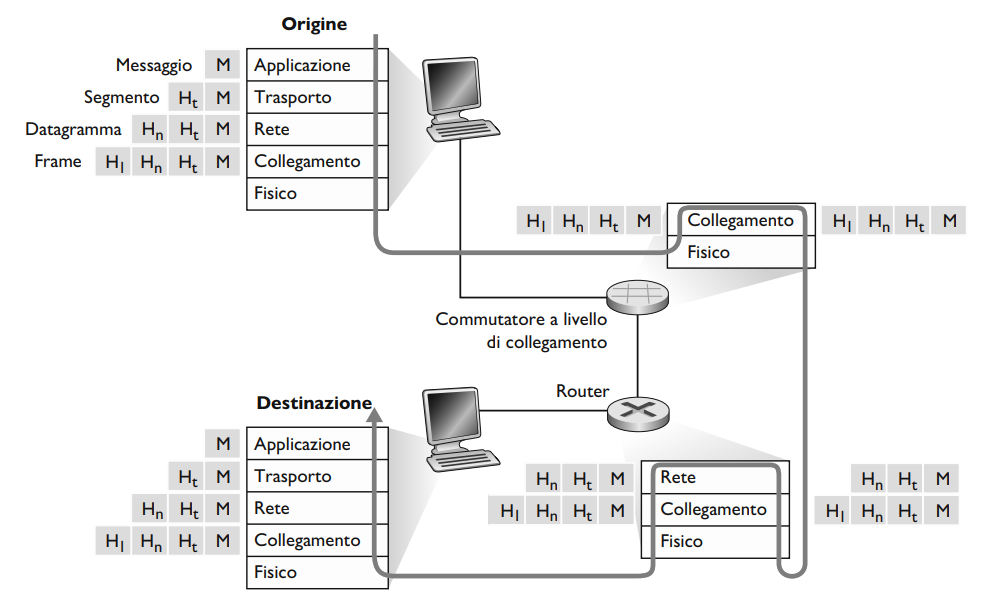
\includegraphics[width=\textwidth, height=6cm, keepaspectratio]{img/stack_protocollare.png}

\subsubsection{Incapsulamento}

L'\textbf{incapsulamento} è il processo mediante il quale i dati vengono avvolti con informazioni di intestazione aggiuntive man mano che si spostano verso il basso nella pila protocollare. Ogni livello aggiunge la propria intestazione, che contiene informazioni di controllo rilevanti per la funzione di quel livello. Questo processo è cruciale per consentire la comunicazione tra i diversi livelli e attraverso reti diverse.

\textbf{Payload:} Il \textit{payload} di un pacchetto è la parte di dati che viene trasportata, ovvero i dati effettivi che il livello superiore vuole trasmettere. Ad esempio, il payload di un segmento TCP è il messaggio del livello applicazione, mentre il payload di un datagramma IP è il segmento TCP.

\begin{itemize}
    \item \textbf{Origine dei Dati al Livello di Applicazione:} Il processo inizia al livello di applicazione, dove vengono generati i dati dell'utente (es. un messaggio email, una richiesta di pagina web). Questi dati sono spesso chiamati "messaggio" e costituiscono il payload per i livelli inferiori.
    \item \textbf{Incapsulamento al Livello di Trasporto:} Il livello di applicazione passa il messaggio al livello di trasporto. Il livello di trasporto aggiunge la propria intestazione al messaggio, creando un "segmento". Questa intestazione contiene informazioni come i numeri di porta, utilizzati per identificare l'applicazione specifica sugli host mittente e destinatario. Il livello di trasporto potrebbe anche aggiungere numeri di sequenza e checksum per una consegna affidabile dei dati (nel caso di TCP). Il payload di questo segmento è il messaggio del livello applicazione.
    \item \textbf{Incapsulamento al Livello di Rete:} Il segmento viene quindi passato al livello di rete. Il livello di rete aggiunge la propria intestazione, creando un "datagramma". Questa intestazione contiene gli indirizzi IP di origine e destinazione, utilizzati per instradare il datagramma attraverso la rete. Il payload di questo datagramma è il segmento del livello di trasporto.
    \item \textbf{Incapsulamento al Livello di Collegamento:} Il datagramma viene passato al livello di collegamento. Il livello di collegamento aggiunge la propria intestazione e coda, creando un "frame". Questa intestazione contiene informazioni come gli indirizzi MAC, utilizzati per consegnare il frame attraverso un singolo collegamento. La coda spesso contiene un checksum per il rilevamento degli errori. Il payload di questo frame è il datagramma del livello di rete.
    \item \textbf{Trasmissione al Livello Fisico:} Infine, il frame viene passato al livello fisico, che trasmette i bit del frame attraverso il mezzo fisico (es. cavo di rame, fibra ottica, segnale wireless).
    \item \textbf{Decapsulamento alla Destinazione:} Quando i dati raggiungono la destinazione, il processo viene invertito. Ogni livello all'estremità ricevente rimuove la propria intestazione corrispondente, passando i dati al livello superiore successivo. Questo processo è chiamato decapsulamento.
\end{itemize}

In sostanza, l'incapsulamento è il processo di avvolgere i dati con intestazioni man mano che si spostano verso il basso nella pila protocollare, consentendo la comunicazione tra i livelli e attraverso le reti. 

